\documentclass[12pt,a4paper]{report}

% ======================== PACKAGES ========================
\usepackage[utf8]{inputenc}
\usepackage[T1]{fontenc}
\usepackage{times}
\usepackage[margin=1in, left=1.25in]{geometry}
\usepackage{graphicx}
\usepackage{float}
\usepackage{array}
\usepackage{longtable}
\usepackage{booktabs}
\usepackage{multirow}
\usepackage{tabularx}
\usepackage{caption}
\usepackage{subcaption}
\usepackage{amsmath}
\usepackage{amssymb}
\usepackage{hyperref}
\usepackage{enumitem}
\usepackage{titlesec}
\usepackage{setspace}
\usepackage{fancyhdr}
\usepackage{tocloft}
\usepackage{xcolor}
\usepackage{tikz}
\usepackage{pdfpages}
\usepackage{textcomp}
\usepackage{url}
\usepackage{cite}
\usepackage{listings}

% ======================== CONFIGURATION ========================
\onehalfspacing
\setlength{\parindent}{1.5em}
\setlength{\parskip}{6pt}

% Hyperlink styling
\hypersetup{
    colorlinks=true,
    linkcolor=black,
    citecolor=blue,
    urlcolor=blue,
    bookmarks=true
}

% Header/Footer
\pagestyle{fancy}
\fancyhf{}
\fancyhead[L]{\small\leftmark}
\fancyhead[R]{\small NutriSense}
\fancyfoot[C]{\thepage}
\renewcommand{\headrulewidth}{0.4pt}
\renewcommand{\footrulewidth}{0pt}

% Chapter title formatting
\titleformat{\chapter}[display]
  {\normalfont\Large\bfseries\centering}
  {\MakeUppercase{\chaptertitlename}\ \thechapter}{12pt}{\LARGE\MakeUppercase}
\titlespacing*{\chapter}{0pt}{-20pt}{20pt}

% Section formatting
\titleformat{\section}{\large\bfseries}{\thesection}{1em}{}
\titleformat{\subsection}{\normalsize\bfseries}{\thesubsection}{1em}{}
\titleformat{\subsubsection}{\normalsize\bfseries\itshape}{\thesubsubsection}{1em}{}

% Graphics path
\graphicspath{{images/}}

% Code listing style
\lstset{
    basicstyle=\small\ttfamily,
    breaklines=true,
    frame=single,
    backgroundcolor=\color{gray!10},
    keywordstyle=\color{blue},
    commentstyle=\color{green!50!black},
    stringstyle=\color{red!70!black},
}

% ======================== DOCUMENT ========================
\begin{document}

% ======================== TITLE PAGE ========================
\begin{titlepage}
\begin{center}
\vspace*{1cm}

{\large\textbf{Savitribai Phule Pune University}}\\[0.5cm]
{\large Sahyadri Valley College of Engineering and Technology, Rajuri,\\Rajuri -- 412411}\\[0.3cm]
{\normalsize Department of Computer Engineering}\\[1.5cm]

\rule{\textwidth}{1.5pt}\\[0.5cm]
{\LARGE\textbf{NutriSense: IoT-Based Health Monitoring and\\AI-Powered Nutrition Advisory System}}\\[0.3cm]
\rule{\textwidth}{1.5pt}\\[1.5cm]

{\large\textbf{A Project Report}}\\[0.3cm]
{\normalsize Submitted in partial fulfillment of the requirements for the award of the degree of}\\[0.3cm]
{\large\textbf{Bachelor of Engineering (Computer Engineering)}}\\[1.5cm]

{\normalsize\textbf{Submitted by}}\\[0.3cm]

\begin{tabular}{|c|c|c|}
\hline
\textbf{Sr. No.} & \textbf{Name of Student} & \textbf{PRN} \\
\hline
1 & Siddhi & 72261481M \\
\hline
2 & Pradnya & 72261503F \\
\hline
3 & Sakshi & 72261452H \\
\hline
\end{tabular}\\[1.5cm]

{\normalsize\textbf{Under the Guidance of}}\\[0.3cm]
{\normalsize Prof. [Guide Name]}\\[2cm]

{\large\textbf{Academic Year 2025--2026}}

\end{center}
\end{titlepage}

% ======================== CERTIFICATE ========================
\newpage
\thispagestyle{empty}
\begin{center}
{\large\textbf{Sahyadri Valley College of Engineering and Technology, Rajuri,\\Rajuri -- 412411}}\\[0.3cm]
{\normalsize Department of Computer Engineering}\\[1.5cm]

\rule{\textwidth}{1.5pt}\\[0.5cm]
{\LARGE\textbf{CERTIFICATE}}\\[0.3cm]
\rule{\textwidth}{1.5pt}\\[1.5cm]
\end{center}

\setlength{\parindent}{2em}
This is to certify that the project entitled \textbf{``NutriSense: IoT-Based Health Monitoring and AI-Powered Nutrition Advisory System''} submitted by \textbf{Siddhi (PRN: 72261481M)}, \textbf{Pradnya (PRN: 72261503F)}, and \textbf{Sakshi (PRN: 72261452H)} in partial fulfillment of the requirements for the award of the degree of \textbf{Bachelor of Engineering in Computer Engineering} from \textbf{Savitribai Phule Pune University} is a record of bonafide work carried out under our supervision and guidance during the academic year 2025--2026.

\vspace{0.5cm}
The matter embodied in this project report has not been submitted for the award of any other degree or diploma.

\vspace{3cm}

\noindent
\begin{minipage}[t]{0.45\textwidth}
\centering
\rule{5cm}{0.4pt}\\
\textbf{Prof. [Guide Name]}\\
Project Guide\\
Dept. of Computer Engineering
\end{minipage}
\hfill
\begin{minipage}[t]{0.45\textwidth}
\centering
\rule{5cm}{0.4pt}\\
\textbf{Prof. Khatal K. B.}\\
Head of Department\\
Dept. of Computer Engineering
\end{minipage}

\vspace{3cm}
\begin{center}
\rule{5cm}{0.4pt}\\
\textbf{Mrs. Balaramudu P.B.}\\
Principal\\
Sahyadri Valley College of Engineering and Technology
\end{center}

\vspace{1cm}
\noindent Date: \rule{3cm}{0.4pt} \hfill Place: Rajuri

% ======================== ACKNOWLEDGEMENT ========================
\newpage
\thispagestyle{empty}
\begin{center}
{\LARGE\textbf{ACKNOWLEDGEMENT}}\\[0.5cm]
\rule{\textwidth}{1pt}
\end{center}
\vspace{1cm}

We wish to express our sincere gratitude to all those who have contributed to the successful completion of this project titled \textbf{``NutriSense: IoT-Based Health Monitoring and AI-Powered Nutrition Advisory System.''}

First and foremost, we extend our deepest thanks to our project guide, \textbf{Prof. [Guide Name]}, Department of Computer Engineering, for their invaluable guidance, consistent encouragement, constructive criticism, and technical expertise throughout the course of this project. Their mentorship has been instrumental in shaping the direction and quality of this work.

We are grateful to \textbf{Prof. Khatal K. B.}, Head of the Department of Computer Engineering, for providing us with the necessary infrastructure and academic support to undertake this project. We also express our heartfelt appreciation to the \textbf{Principal, Mrs. Balaramudu P.B.}, for fostering a conducive academic environment at Sahyadri Valley College of Engineering and Technology, Rajuri.

We extend our thanks to all the faculty members of the Department of Computer Engineering whose teachings and insights during our undergraduate program have laid the foundation for the technical skills applied in this project. The knowledge gained in courses pertaining to software engineering, database management, web technologies, artificial intelligence, and IoT systems has been directly instrumental in the realization of NutriSense.

We acknowledge the contributions of the open-source community, particularly the developers of React.js, Node.js, Express.js, MongoDB, Flask, MediaPipe, and Flutter, whose robust and well-documented frameworks made it possible to construct a complex multi-tier application within an academic timeline. We also thank Groq Inc. for providing API access to their high-performance LLaMA model inference platform, which powers the AI advisory capabilities of this system.

Finally, we are immensely grateful to our families and friends for their unwavering support, patience, and encouragement throughout this endeavour.

\vspace{1.5cm}
\begin{flushright}
\textbf{--- Siddhi, Pradnya, Sakshi}\\
Rajuri, April 2026
\end{flushright}

% ======================== ABSTRACT ========================
\newpage
\thispagestyle{empty}
\begin{center}
{\LARGE\textbf{ABSTRACT}}\\[0.5cm]
\rule{\textwidth}{1pt}
\end{center}
\vspace{0.5cm}

The exponential growth of lifestyle-related diseases --- including diabetes, hypertension, cardiovascular disorders, and obesity --- has underscored an urgent need for proactive, technology-driven health monitoring solutions that empower individuals with real-time insights into their physiological well-being and nutritional habits. Existing health monitoring platforms suffer from significant fragmentation: wearable devices track vitals in isolation, nutrition applications operate independently without clinical context, and medical advisory systems rely on sporadic physician consultations rather than continuous data-driven analysis.

\textbf{NutriSense} is a comprehensive, full-stack IoT-based health monitoring and AI-powered nutrition advisory system designed to bridge this gap by unifying contactless physiological sensing, intelligent nutritional analysis, and personalized health advisory within a single integrated platform. The system employs \textbf{Remote Photoplethysmography (rPPG)} technology, implemented through Google's MediaPipe face detection framework and Fast Fourier Transform (FFT) signal processing, to perform contactless heart rate monitoring, Heart Rate Variability (HRV) estimation, and stress scoring via a standard webcam --- eliminating the need for dedicated wearable hardware.

The platform provides \textbf{multi-modal meal logging} capabilities including text-based nutritional analysis optimized for Indian cuisine, voice input via the browser-native Web Speech API, AI-powered food photo recognition using the Groq LLaMA 4 Scout vision model, and a novel portion size estimation system employing reference objects (credit cards, coins, hands) for accurate gram-level food quantification. An AI Doctor chatbot powered by Groq LLaMA 3.3 70B provides personalized, vitals-aware health advisory, while a \textbf{Retrieval-Augmented Generation (RAG)} diet chatbot enriches responses with curated nutritional knowledge and the user's historical health data.

The system further implements a rule-based diet recommendation engine, a four-dimensional health risk assessment engine (Diabetes, Hypertension, Heart Disease, Obesity), BMI body composition analysis with Mifflin-St Jeor basal metabolic rate calculation, and a gamification engine with experience points, badges, streaks, and challenges to sustain user engagement.

NutriSense is architected as a multi-tier distributed system comprising a \textbf{React 19} single-page application with Vite build tooling, a \textbf{Node.js Express 5} RESTful backend, \textbf{MongoDB Atlas} cloud database, a \textbf{Python Flask} IoT processing server, and a \textbf{Flutter} cross-platform mobile application.

\vspace{0.5cm}
\noindent\textbf{Keywords:} IoT, Remote Photoplethysmography, Health Monitoring, Artificial Intelligence, LLM, Nutrition Analysis, MERN Stack, MediaPipe, Groq, Gamification

% ======================== TABLE OF CONTENTS ========================
\newpage
\tableofcontents

% ======================== LIST OF FIGURES ========================
\newpage
\listoffigures

% ======================== LIST OF TABLES ========================
\newpage
\listoftables

% ======================== CHAPTER 1 ========================
\chapter{Introduction and Project Scope}
\pagenumbering{arabic}

\section{Introduction}
The twenty-first century has witnessed an unprecedented convergence of information technology and healthcare, driven by the proliferation of Internet of Things (IoT) devices, advancements in artificial intelligence, and the growing accessibility of cloud computing infrastructure. The World Health Organization has identified non-communicable diseases (NCDs) --- including cardiovascular diseases, diabetes mellitus, chronic respiratory conditions, and obesity-related disorders --- as the leading cause of global mortality, accounting for approximately 74\% of all deaths worldwide. In India specifically, the rapid urbanization and accompanying shifts in dietary patterns and sedentary lifestyles have led to alarming increases in the prevalence of lifestyle diseases, with the Indian Council of Medical Research estimating that over 101 million Indians are currently living with diabetes and an additional 136 million in a pre-diabetic state.

Traditional healthcare delivery models operate on a reactive paradigm, where patients seek medical intervention only after the manifestation of symptomatic illness. This approach inherently limits the potential for early detection and preventive intervention, which are universally acknowledged as the most cost-effective strategies for combating chronic diseases. The advent of IoT-enabled health monitoring systems has introduced a new paradigm of continuous, real-time physiological surveillance that holds the promise of transitioning healthcare from reactive treatment to proactive prevention. However, the current landscape of digital health solutions suffers from severe fragmentation: wearable fitness trackers monitor heart rate and activity in isolation from dietary context, nutrition tracking applications require tedious manual food logging without correlation to physiological data, and medical advisory services remain disconnected from the continuous data streams generated by both categories of tools.

This fragmentation creates a critical void in the patient's health management journey. A user who monitors their heart rate through a smartwatch receives no guidance on how their dietary choices impact their cardiovascular metrics. Conversely, a user who diligently logs their meals in a nutrition application receives no feedback on how their food intake affects their blood pressure, glucose levels, or stress indicators.

The NutriSense system has been conceived and developed to address this fundamental gap. NutriSense is a comprehensive, full-stack IoT-based health monitoring and AI-powered nutrition advisory system that seamlessly unifies contactless vital sign sensing, multi-modal intelligent nutritional analysis, personalized AI health advisory, and behavioural gamification within an integrated web and mobile platform. By correlating real-time physiological data with detailed nutritional intake data, NutriSense delivers a uniquely holistic health management experience that no existing consumer platform currently offers.

\section{Problem Statement}
Despite the proliferation of health monitoring wearables and nutrition tracking applications, there exists no integrated platform that correlates real-time physiological vital signs with dietary intake data to deliver personalized, AI-driven health and nutrition advisory. Current solutions operate in isolation --- fitness devices monitor vitals without dietary context, nutrition apps track food without physiological correlation, and medical advisory remains fragmented and episodic. There is a pressing need for a unified system that performs contactless health monitoring via accessible hardware (webcam), provides multi-modal nutrition tracking (text, voice, image), correlates health and nutrition data through AI-powered analysis, and delivers personalized, continuous advisory --- all within a single, gamified platform accessible via web and mobile interfaces.

\section{Motivation}
The motivation for developing NutriSense stems from several converging factors:

\textbf{Rising Burden of Lifestyle Diseases:} India is experiencing an epidemiological transition, with NCDs now surpassing infectious diseases as the primary cause of morbidity and mortality. The National Family Health Survey (NFHS-5) reveals that 24\% of Indian adults are overweight or obese, while the prevalence of diabetes has risen to 15.3\% in urban areas.

\textbf{Democratization of AI and LLM Technology:} The emergence of open-weight Large Language Models, particularly Meta's LLaMA family, and high-performance inference platforms such as Groq, has democratized access to sophisticated natural language understanding and generation capabilities at negligible marginal cost per interaction.

\textbf{Accessibility of Contactless Sensing:} The maturation of Remote Photoplethysmography (rPPG) technology presents an opportunity to perform contactless heart rate monitoring using nothing more than a laptop webcam, eliminating hardware barriers and making health monitoring universally accessible.

\section{Project Objectives}
The objectives of the NutriSense project have been formally categorized into three tiers:

\textbf{Necessary Requirements (NR):}
\begin{itemize}[leftmargin=2cm]
  \item[\textbf{NR1:}] Implement contactless heart rate monitoring via Remote Photoplethysmography (rPPG) using a standard webcam, Google MediaPipe face detection, and Fast Fourier Transform (FFT) signal processing, with HRV estimation and stress scoring.
  \item[\textbf{NR2:}] Develop multi-modal meal logging supporting text-based nutritional analysis, voice input via Web Speech API (en-IN locale), and AI-powered food photo recognition using Groq LLaMA 4 Scout vision model.
  \item[\textbf{NR3:}] Integrate the Groq LLaMA Large Language Model family for personalized AI health advisory, including an AI Doctor chatbot, diet plan generation, and meal analysis.
  \item[\textbf{NR4:}] Build a comprehensive, four-dimensional health risk assessment engine that correlates physiological vital signs with nutritional intake patterns.
\end{itemize}

\textbf{Expected Requirements (EXP):}
\begin{itemize}[leftmargin=2cm]
  \item[\textbf{EXP1:}] Deploy a real-time health dashboard with computed health scores (0--100), vital sign trend visualization, and smart alert generation.
  \item[\textbf{EXP2:}] Implement a gamification engine with experience points (XP), 11 progression levels, 7 achievement badges, and streak tracking.
  \item[\textbf{EXP3:}] Develop an AI-powered portion size estimation module using reference object comparison.
\end{itemize}

\textbf{Exciting Requirements (EXC):}
\begin{itemize}[leftmargin=2cm]
  \item[\textbf{EXC1:}] Enable cross-platform mobile access via a Flutter application.
  \item[\textbf{EXC2:}] Implement a Retrieval-Augmented Generation (RAG) diet chatbot with curated knowledge base.
\end{itemize}

\section{Scope of the Project}
The NutriSense system encompasses sixteen functional modules: (1)~User Authentication, (2)~Health Dashboard, (3)~rPPG Heart Rate Scanner, (4)~Manual Vitals Logging, (5)~BMI Tracker \& Body Composition, (6)~AI Diet Plan, (7)~Meal Logger, (8)~Food Photo Scanner, (9)~Portion Size Estimator, (10)~AI Doctor Chatbot, (11)~RAG Diet AI Chatbot, (12)~Health Risk Assessment, (13)~Health History \& Visualization, (14)~Gamification \& Rewards, (15)~User Profile, and (16)~Flutter Mobile Application.

\section{Real-World Impact}
In the domain of \textbf{preventive healthcare}, NutriSense shifts the paradigm from reactive medical consultation to continuous, proactive health monitoring. With respect to \textbf{nutritional awareness}, NutriSense addresses a critical gap in health literacy, particularly in the Indian context where traditional dietary assessment tools are poorly calibrated for regional cuisines. The \textbf{accessibility} of the platform --- requiring only a web browser and webcam --- dramatically lowers the barrier to health monitoring. The \textbf{gamification layer} addresses the critical challenge of sustained user engagement.

% ======================== CHAPTER 2 ========================
\chapter{Literature Survey}

\section{Introduction to Literature Review}
The development of NutriSense is informed by a substantial body of prior work spanning IoT-based health monitoring, AI-powered food recognition, machine learning-driven health risk prediction, and contactless vital sign sensing. This literature survey systematically reviews five representative works and establishes the differentiation for the NutriSense approach.

\section{Review of Past Systems}

\subsection{Sharma et al. (2019) --- IoT-Based Health Monitoring System Using Raspberry Pi}
Sharma, Kumar, and Singh \cite{sharma2019} presented an IoT-based health monitoring framework built around the Raspberry Pi single-board computer, interfaced with dedicated biomedical sensors including a pulse oximeter (MAX30102), temperature sensor (DS18B20), and ECG module (AD8232). The system transmitted sensor readings to a cloud server via Wi-Fi. The primary contribution lay in demonstrating low-cost, Raspberry Pi-based health monitoring. However, the system suffered from reliance on wired contact-based sensors, absence of nutritional analysis, no AI component, and a basic web dashboard. NutriSense addresses these through contactless rPPG sensing, integrated AI nutrition analysis, and a comprehensive gamified experience.

\subsection{Singh and Kumar (2020) --- Smart Health Monitoring using IoT and Cloud}
Singh and Kumar \cite{singh2020} proposed a cloud-integrated smart health monitoring system utilizing Arduino with heartbeat, temperature, and accelerometer sensors, transmitting data to ThingSpeak IoT cloud. Despite threshold-based alerting and 99.2\% data reliability, the system lacked contextual intelligence, dietary advisory, and required dedicated hardware. NutriSense transcends these through AI-powered contextual analysis and hardware-free contactless sensing.

\subsection{Harshitha et al. (2021) --- AI-Based Food Recognition and Calorie Estimation}
Harshitha, Priya, and Lakshmi \cite{harshitha2021} developed a CNN-based food recognition system using fine-tuned VGG-16, achieving 78.3\% top-1 accuracy on 50 food categories. Limitations included single-modality (image-only), no portion size estimation, no health correlation, and Western food bias. NutriSense addresses these with multi-modal logging, reference-object portion estimation, health-nutrition correlation, and Indian food optimization.

\subsection{Yadav and Sharma (2022) --- ML-based Health Risk Prediction}
Yadav and Sharma \cite{yadav2022} presented an ensemble ML system (Random Forest, Gradient Boosting, SVM) for health risk prediction, achieving F1-score of 0.87 for cardiovascular risk. Limitations included requirement for laboratory blood tests, no intervention recommendations, Western dataset bias, and no IoT component. NutriSense computes risk from daily app interaction data without clinical testing.

\subsection{Patel et al. (2023) --- Remote Photoplethysmography for Contactless Vital Sign Monitoring}
Patel, Chen, and Williams \cite{patel2023} authored a comprehensive rPPG review, identifying $\pm$2--5 BPM accuracy under controlled conditions. No system reviewed integrated rPPG with nutritional analysis. NutriSense demonstrates one of the first practical integrations of rPPG with AI-powered nutrition analysis.

\section{Comparative Analysis}

\begin{table}[H]
\centering
\caption{Comparative Analysis of Existing Systems vs. NutriSense}
\label{tab:comparison}
\small
\begin{tabular}{|l|c|c|c|c|c|c|}
\hline
\textbf{Feature} & \textbf{Sharma} & \textbf{Singh} & \textbf{Harshitha} & \textbf{Yadav} & \textbf{Patel} & \textbf{NutriSense} \\
\hline
IoT Integration & \checkmark & \checkmark & $\times$ & $\times$ & \checkmark & \checkmark \\
Contactless & $\times$ & $\times$ & $\times$ & $\times$ & \checkmark & \checkmark \\
AI/LLM & $\times$ & $\times$ & CNN & ML & $\times$ & \textbf{4 LLMs} \\
Nutrition & $\times$ & $\times$ & Image & $\times$ & $\times$ & \textbf{Multi-modal} \\
Diet Advisory & $\times$ & $\times$ & $\times$ & $\times$ & $\times$ & \checkmark \\
Correlation & $\times$ & $\times$ & $\times$ & $\times$ & $\times$ & \checkmark \\
Voice Input & $\times$ & $\times$ & $\times$ & $\times$ & $\times$ & \checkmark \\
Gamification & $\times$ & $\times$ & $\times$ & $\times$ & $\times$ & \checkmark \\
Mobile App & $\times$ & $\times$ & $\times$ & Web & $\times$ & \checkmark \\
Indian Food & $\times$ & $\times$ & $\times$ & $\times$ & $\times$ & \checkmark \\
\hline
\end{tabular}
\end{table}

\section{Research Gaps Identified}
\begin{enumerate}
  \item \textbf{Absence of Health-Nutrition Integration} --- No reviewed system correlates vital signs with dietary data.
  \item \textbf{Hardware Dependency} --- IoT systems require dedicated sensor hardware.
  \item \textbf{Single-Modality Nutrition Tracking} --- Only image-based food recognition exists.
  \item \textbf{Lack of Conversational Advisory} --- No personalized, LLM-powered health advisory.
  \item \textbf{Absence of Engagement Mechanisms} --- No gamification in health monitoring systems.
  \item \textbf{Limited Regional Food Coverage} --- Western food database bias.
\end{enumerate}

\section{Conclusion of Literature Survey}
The literature survey establishes that no existing system integrates contactless rPPG monitoring, multi-modal AI nutrition analysis, LLM-powered health advisory, and gamified engagement within a single platform. NutriSense addresses all identified gaps.

% ======================== CHAPTER 3 ========================
\chapter{Dissertation Plan and Project Estimation}

\section{Work Breakdown Structure}

\begin{table}[H]
\centering
\caption{Work Breakdown Structure (T1--T8)}
\label{tab:wbs}
\begin{tabular}{|c|p{8cm}|c|c|}
\hline
\textbf{Task ID} & \textbf{Task Description} & \textbf{Duration} & \textbf{Dependencies} \\
\hline
T1 & Requirements Analysis \& System Design & 2 weeks & --- \\
T2 & Database Schema Design \& Backend Architecture & 2 weeks & T1 \\
T3 & Authentication \& User Management & 1 week & T2 \\
T4 & IoT rPPG Module --- MediaPipe + Flask Server & 3 weeks & T1 \\
T5 & Frontend Development --- React Dashboard \& Modules & 4 weeks & T3, T4 \\
T6 & AI Integration --- Groq LLM, Vision, RAG & 3 weeks & T2 \\
T7 & Mobile App Development --- Flutter & 2 weeks & T3 \\
T8 & Testing, Integration \& Deployment & 2 weeks & T5, T6, T7 \\
\hline
\end{tabular}
\end{table}

\section{COCOMO Estimation}

\subsection{Lines of Code Estimation}
\begin{table}[H]
\centering
\caption{COCOMO Estimation Parameters}
\label{tab:cocomo}
\begin{tabular}{|l|l|c|}
\hline
\textbf{Component} & \textbf{Technology} & \textbf{KLOC} \\
\hline
Backend (server, controllers, models, routes, services) & Node.js & 2.5 \\
Frontend (16 pages, 3 components, context, services, CSS) & React/JSX/CSS & 8.0 \\
IoT Server (mediapipe\_server.py) & Python & 0.5 \\
Mobile App (Flutter) & Dart & 0.2 \\
\hline
\textbf{Total} & & \textbf{11.2} \\
\hline
\end{tabular}
\end{table}

\subsection{COCOMO Calculations (Organic Model)}
The Basic COCOMO Organic model coefficients are: $a = 2.4$, $b = 1.05$, $c = 2.5$, $d = 0.38$.

\textbf{Effort:}
\begin{equation}
E = a \times (KLOC)^b = 2.4 \times (11.2)^{1.05} = 2.4 \times 12.64 = \boxed{30.34 \text{ person-months}}
\end{equation}

\textbf{Development Time:}
\begin{equation}
D = c \times (E)^d = 2.5 \times (30.34)^{0.38} = 2.5 \times 3.66 = \boxed{9.15 \text{ months}}
\end{equation}

\textbf{Average Staff Size:}
\begin{equation}
SS = \frac{E}{D} = \frac{30.34}{9.15} = \boxed{3 \text{ persons}}
\end{equation}

\textbf{Productivity:}
\begin{equation}
P = \frac{KLOC}{E} = \frac{11.2}{30.34} = \boxed{369 \text{ LOC/person-month}}
\end{equation}

\section{Resource Allocation}
\begin{table}[H]
\centering
\caption{Resource Allocation Matrix}
\label{tab:resources}
\begin{tabular}{|l|l|l|}
\hline
\textbf{Category} & \textbf{Resource} & \textbf{Specification} \\
\hline
Hardware & Development Laptops & 3$\times$ (Intel i5, 8GB RAM, 256GB SSD) \\
Hardware & Webcam & Integrated laptop webcam (720p+) \\
Software & Frontend & React 19.2, Vite 8.0, Tailwind CSS 3.4 \\
Software & Backend & Node.js 22, Express.js 5.2, Mongoose 9.2 \\
Software & Database & MongoDB Atlas (M0 Free Tier) \\
Software & IoT Server & Python 3.12, Flask, MediaPipe, OpenCV \\
Software & Mobile & Flutter 3.11, Dart \\
Software & AI Platform & Groq API (LLaMA 3.1/3.3/4 models) \\
Cloud & Hosting & Render (Free Tier) \\
\hline
\end{tabular}
\end{table}

% ======================== CHAPTER 4 ========================
\chapter{Software Requirement Specification}

\section{Mathematical System Definition}
The NutriSense system is formally defined as:
\begin{equation}
S = \{I, P, O, F, DD, NDD\}
\end{equation}

\textbf{Input Set} $I = \{I_1, I_2, \ldots, I_9\}$: User credentials, vital signs, webcam frames, meal text, voice input, food images, reference objects, chat messages, BMI parameters.

\textbf{Processing Set} $P = \{P_1, P_2, \ldots, P_8\}$: JWT authentication, rPPG FFT analysis, rule-based diet engine, Groq LLM inference, health risk scoring, gamification engine, BMI body composition, RAG retrieval pipeline.

\textbf{Output Set} $O = \{O_1, O_2, \ldots, O_8\}$: Health dashboard, rPPG results, nutrition breakdown, AI chat responses, risk assessment, BMI analysis, gamification stats, diet plans.

\section{Functional Requirements}

\begin{table}[H]
\centering
\caption{Functional Requirements Specification}
\label{tab:funcreq}
\small
\begin{tabular}{|c|p{3cm}|p{7cm}|c|}
\hline
\textbf{ID} & \textbf{Requirement} & \textbf{Description} & \textbf{Priority} \\
\hline
FR1 & User Registration & Register with bcrypt hashing, auto BMI calculation & High \\
FR2 & User Authentication & JWT tokens with 7-day expiry, persistent sessions & High \\
FR3 & rPPG Heart Rate & MediaPipe face detection, FFT, $\pm$5 BPM accuracy & High \\
FR4 & Manual Vitals & Accept HR, BP, glucose, SpO2 with AI analysis & High \\
FR5 & Text Meal Analysis & Groq LLaMA analysis returning macros, health score & High \\
FR6 & Voice Meal Input & Web Speech API (en-IN) transcription + analysis & Medium \\
FR7 & Food Photo Scan & LLaMA 4 Scout vision with allergen detection & High \\
FR8 & Portion Estimation & Reference object comparison + density tables & Medium \\
FR9 & AI Doctor Chat & LLaMA 3.3 70B with real-time vitals context & High \\
FR10 & Health Risk & 4-dimensional risk from 14-day data & Medium \\
FR11 & Gamification & XP, levels, badges, streaks, challenges & Low \\
FR12 & BMI Composition & BMI, body fat, BMR, TDEE, macro targets & Medium \\
\hline
\end{tabular}
\end{table}

\section{Non-Functional Requirements}

\begin{table}[H]
\centering
\caption{Non-Functional Requirements Specification}
\label{tab:nfr}
\begin{tabular}{|c|l|p{8cm}|}
\hline
\textbf{ID} & \textbf{Category} & \textbf{Requirement} \\
\hline
NFR1 & Performance & API response $\leq$ 3s standard, $\leq$ 5s AI endpoints \\
NFR2 & Security & bcrypt (salt $\geq$ 10), JWT authentication on all endpoints \\
NFR3 & Usability & Framer Motion animations, responsive layouts \\
NFR4 & Reliability & Graceful AI failure handling with fallback responses \\
NFR5 & Scalability & MongoDB Atlas + Render cloud horizontal scaling \\
NFR6 & Portability & Cross-browser (Chrome, Firefox, Edge, Safari) + mobile \\
\hline
\end{tabular}
\end{table}

\section{RMMM Risk Analysis}

\begin{table}[H]
\centering
\caption{RMMM Risk Analysis Table}
\label{tab:rmmm}
\small
\begin{tabular}{|c|p{4cm}|c|c|p{4.5cm}|}
\hline
\textbf{ID} & \textbf{Description} & \textbf{Prob.} & \textbf{Impact} & \textbf{Mitigation} \\
\hline
R1 & rPPG deviation $>$10 BPM & 40\% & High & Multi-FPS fallback, 45-180 BPM validation \\
R2 & AI hallucination & 30\% & Medium & JSON parsing, medical disclaimers, rule fallback \\
R3 & Health data exposure & 20\% & Critical & JWT, bcrypt, env variables, HTTPS \\
R4 & Cross-browser webcam issues & 35\% & Medium & Standard getUserMedia(), feature detection \\
R5 & Groq API rate limiting & 50\% & Medium & Request queuing, cached fallbacks \\
\hline
\end{tabular}
\end{table}

% ======================== CHAPTER 5 ========================
\chapter{Detailed Design Documentation}

\section{System Architecture}
The NutriSense system is architected as a multi-tier, distributed application comprising six distinct layers: Client Layer (React 19 SPA + Flutter), Server Layer (Node.js Express 5), IoT Processing Layer (Python Flask + MediaPipe), Database Layer (MongoDB Atlas), AI Layer (Groq LLaMA models), and Mobile Layer (Flutter).

\begin{figure}[H]
\centering
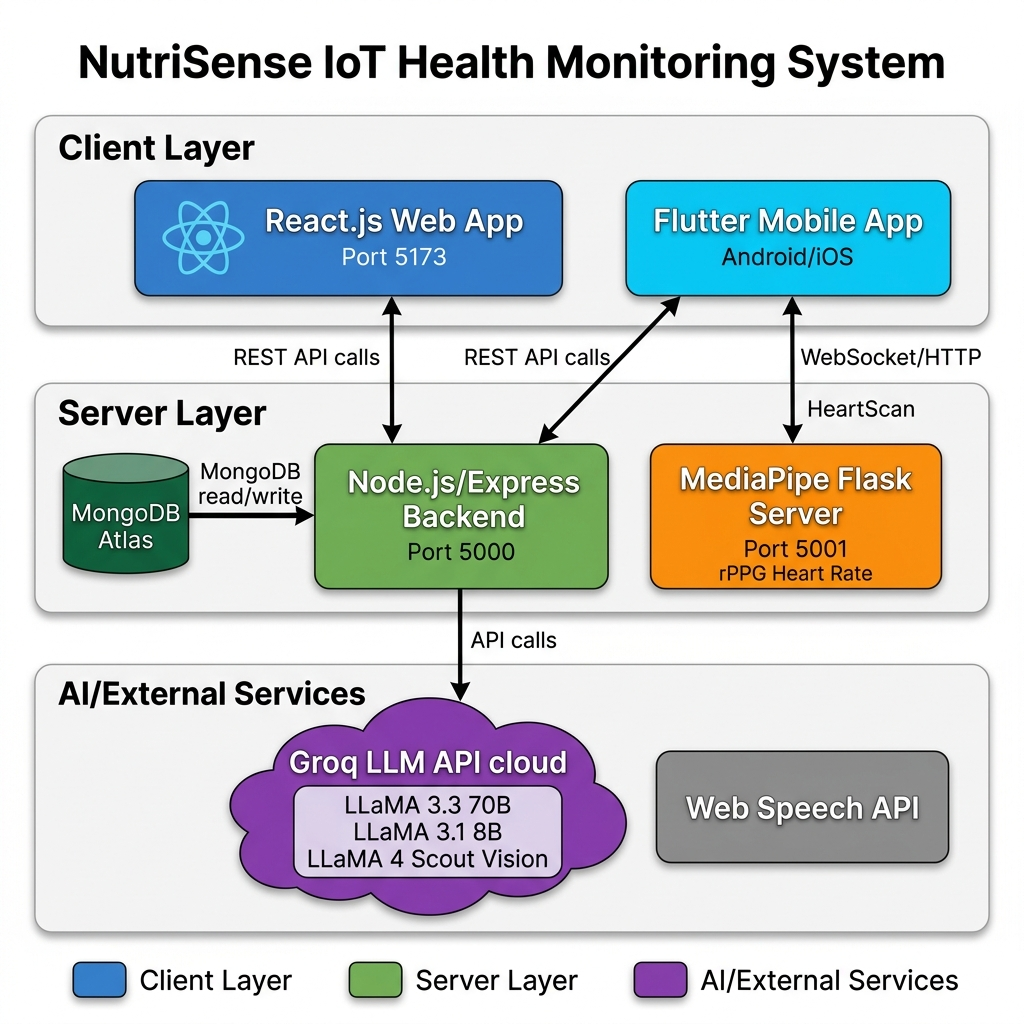
\includegraphics[width=0.95\textwidth]{system_architecture_1779469815401.png}
\caption{NutriSense System Architecture Diagram}
\label{fig:sysarch}
\end{figure}

\section{Data Processing Engines}

\subsection{rPPG Signal Processing Pipeline}
The rPPG module performs contactless heart rate measurement through six stages:
\begin{enumerate}
  \item \textbf{Face Detection:} MediaPipe short-range detection ($\text{confidence} = 0.4$)
  \item \textbf{Forehead ROI:} Top 5--35\% vertical, 15--85\% horizontal of face bounding box
  \item \textbf{Green Channel:} DC removal and normalization
  \item \textbf{Hanning Window:}
  \begin{equation}
    w(n) = 0.5 \left(1 - \cos\left(\frac{2\pi n}{N-1}\right)\right)
  \end{equation}
  \item \textbf{FFT (4x zero-padded):}
  \begin{equation}
    X(k) = \sum_{n=0}^{N-1} x(n) \cdot e^{-j2\pi kn/N}
  \end{equation}
  Band-pass: 0.75--3.0 Hz (45--180 BPM)
  \item \textbf{Peak Detection:}
  \begin{equation}
    HR = f_{peak} \times 60 \text{ BPM}
  \end{equation}
\end{enumerate}

HRV and stress are computed as:
\begin{equation}
HRV = \sigma(g) \times 2.5 \quad (\text{clamped } [10, 120] \text{ ms})
\end{equation}
\begin{equation}
Stress = 100 - \frac{HRV}{120} \times 100
\end{equation}

\subsection{AI Model Integration}

\begin{table}[H]
\centering
\caption{Groq AI Model Integration Summary}
\label{tab:aimodels}
\begin{tabular}{|l|l|l|}
\hline
\textbf{Feature} & \textbf{Groq Model} & \textbf{Purpose} \\
\hline
Diet Advice & llama-3.1-8b-instant & Personalized diet from vitals \\
AI Doctor Chat & llama-3.3-70b-versatile & Conversational health assistant \\
Meal Text Analysis & llama3-8b-8192 & Nutrition estimation from text \\
Food Photo Scan & llama-4-scout-17b-16e & Vision: food identification \\
Portion Estimation & llama-4-scout-17b-16e & Vision: portion size \\
RAG Diet Chat & llama-3.3-70b-versatile & Knowledge-augmented nutrition \\
\hline
\end{tabular}
\end{table}

\subsection{Gamification Engine}

\begin{table}[H]
\centering
\caption{Gamification XP and Level System}
\label{tab:gamification}
\begin{tabular}{|c|l|c||c|l|c|}
\hline
\textbf{Level} & \textbf{Rank} & \textbf{XP} & \textbf{Level} & \textbf{Rank} & \textbf{XP} \\
\hline
1 & Nutrition Beginner & 0 & 7 & Diet Master & 2200 \\
2 & Health Tracker & 100 & 8 & Wellness Expert & 3000 \\
3 & Diet Explorer & 300 & 9 & Nutrition Guru & 4000 \\
4 & Wellness Warrior & 600 & 10 & Health Legend & 5500 \\
5 & Nutrition Pro & 1000 & 11 & Wellness Titan & 7500 \\
6 & Health Champion & 1500 & & & \\
\hline
\end{tabular}
\end{table}

\section{UML Diagrams}

\begin{figure}[H]
\centering
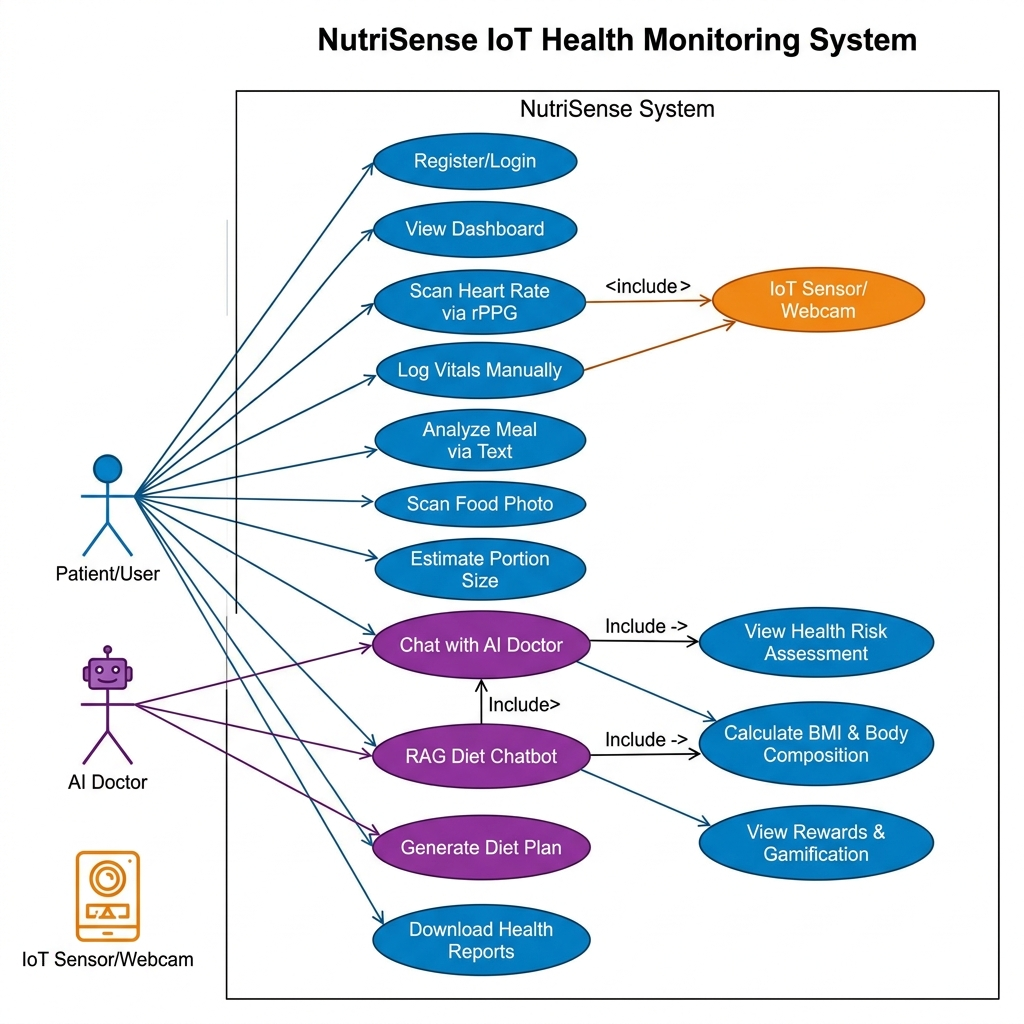
\includegraphics[width=0.9\textwidth]{use_case_diagram_1779469829562.png}
\caption{Use Case Diagram}
\label{fig:usecase}
\end{figure}

\begin{figure}[H]
\centering
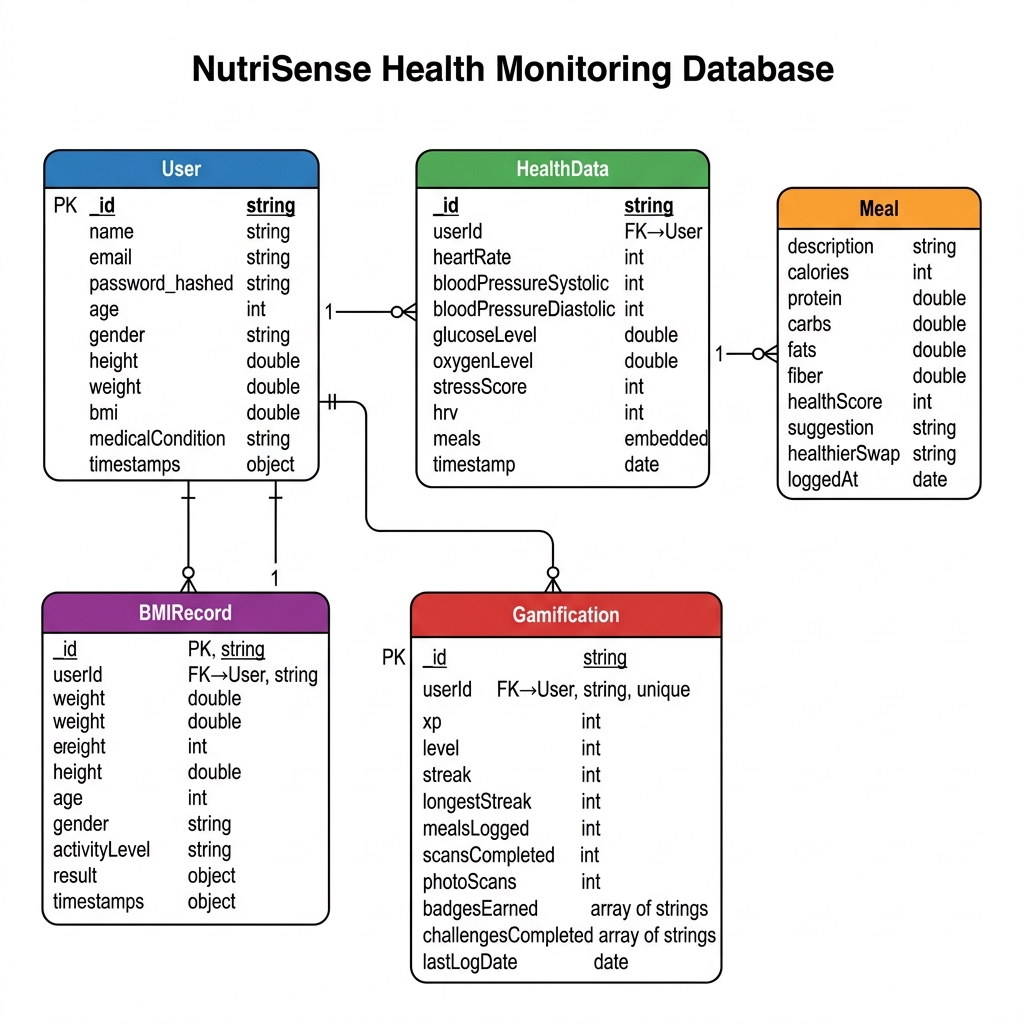
\includegraphics[width=0.9\textwidth]{er_diagram_1779469844207.png}
\caption{Entity-Relationship (ER) Diagram}
\label{fig:erdiagram}
\end{figure}

\begin{figure}[H]
\centering
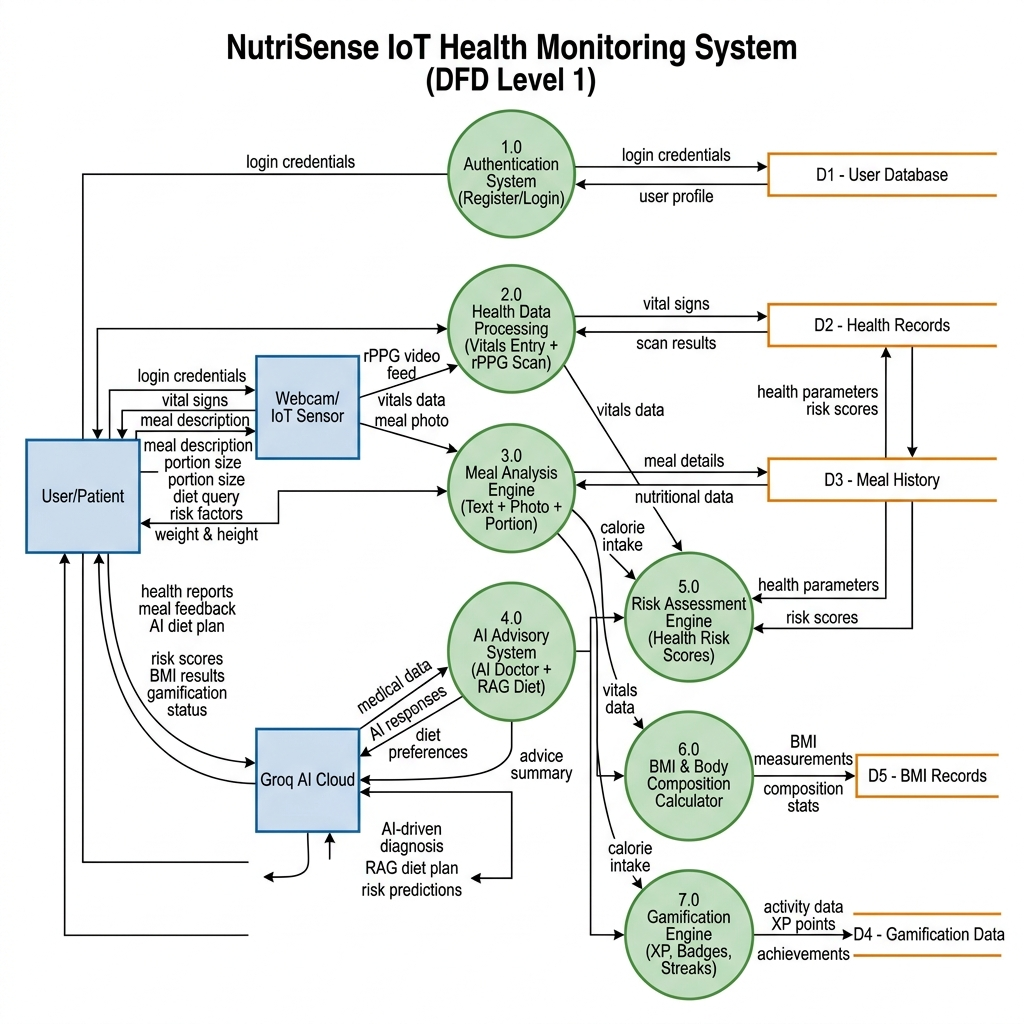
\includegraphics[width=0.9\textwidth]{data_flow_diagram_1779469919176.png}
\caption{Data Flow Diagram (DFD Level 1)}
\label{fig:dfd}
\end{figure}

\begin{figure}[H]
\centering
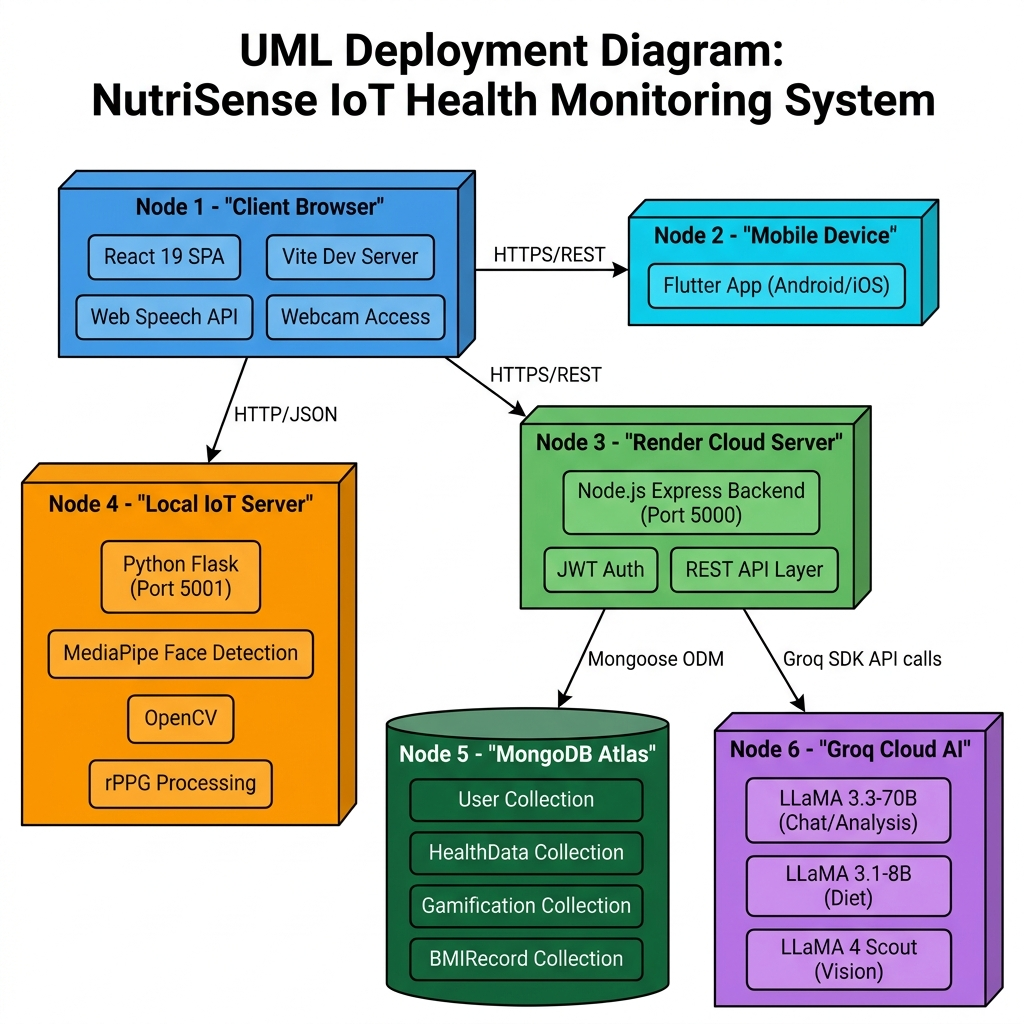
\includegraphics[width=0.9\textwidth]{deployment_diagram_1779469903315.png}
\caption{Deployment Diagram}
\label{fig:deployment}
\end{figure}

\begin{figure}[H]
\centering
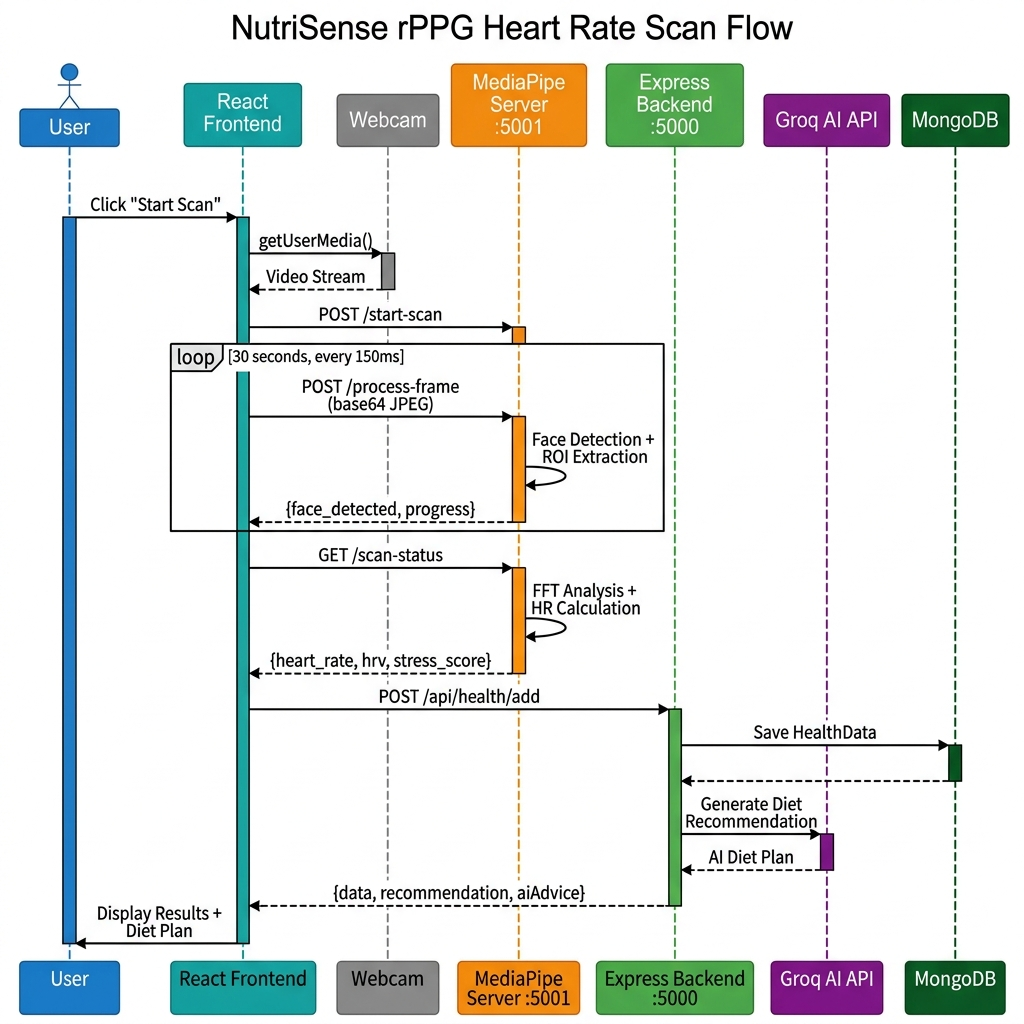
\includegraphics[width=0.9\textwidth]{sequence_diagram_1779469933432.png}
\caption{Sequence Diagram --- rPPG Heart Rate Scan Flow}
\label{fig:sequence}
\end{figure}

\begin{figure}[H]
\centering
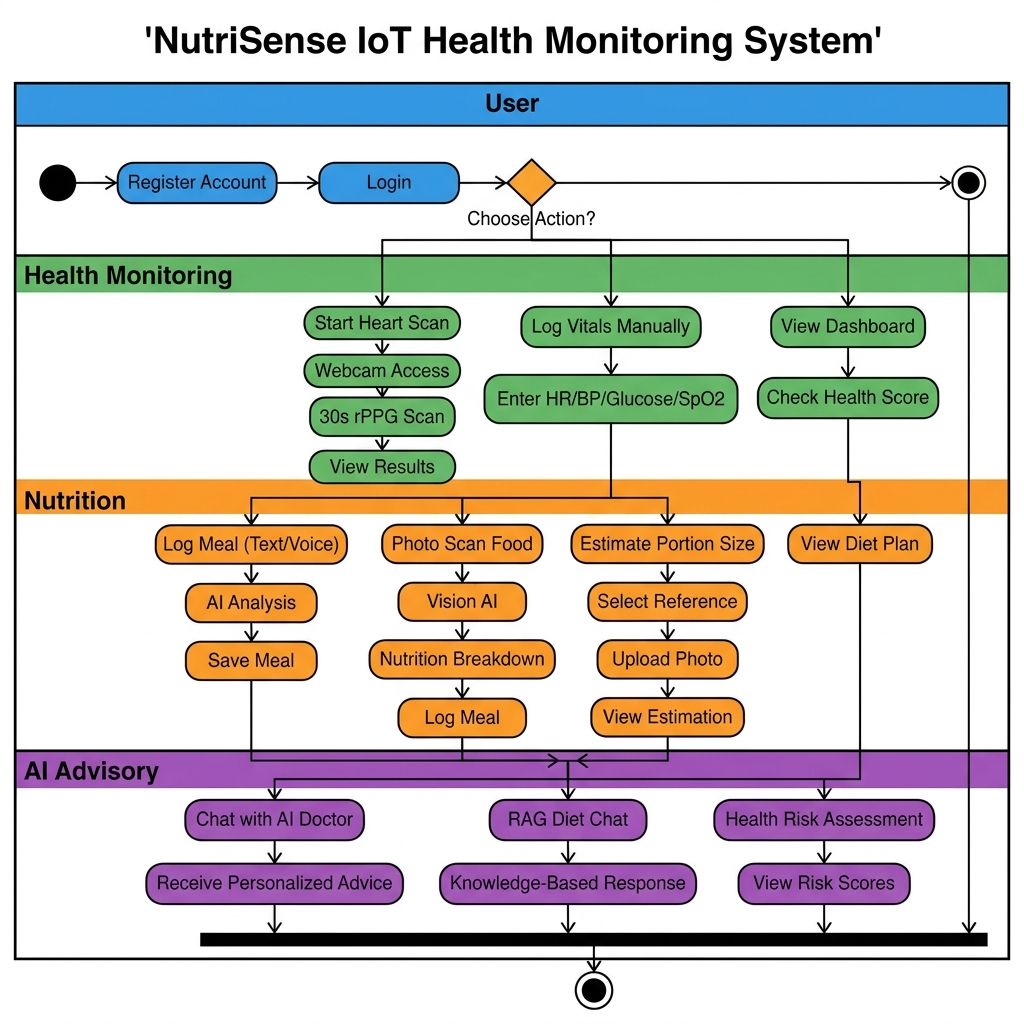
\includegraphics[width=0.9\textwidth]{activity_diagram_1779469984140.png}
\caption{Activity Diagram --- User Workflow}
\label{fig:activity}
\end{figure}

\begin{figure}[H]
\centering
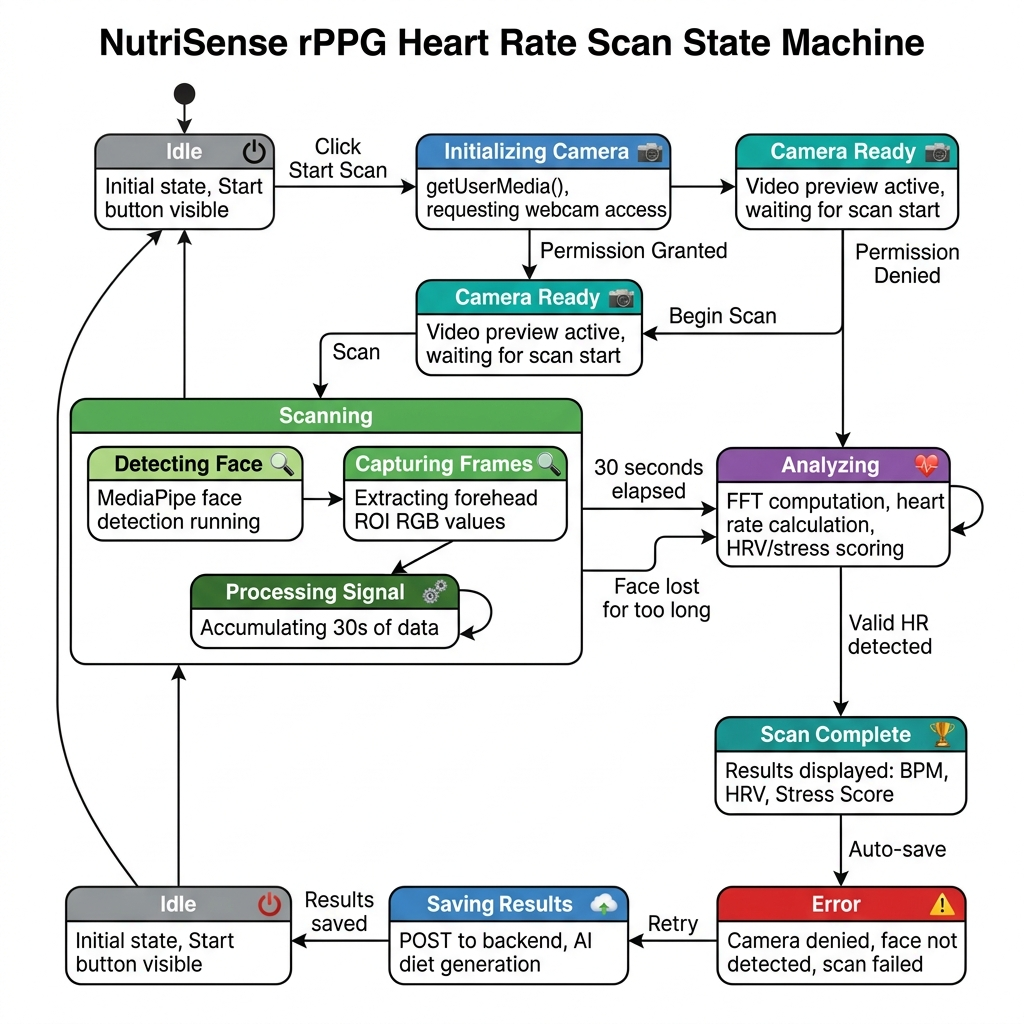
\includegraphics[width=0.9\textwidth]{state_diagram_1779470010013.png}
\caption{State Transition Diagram --- Heart Rate Scan}
\label{fig:state}
\end{figure}

\begin{figure}[H]
\centering
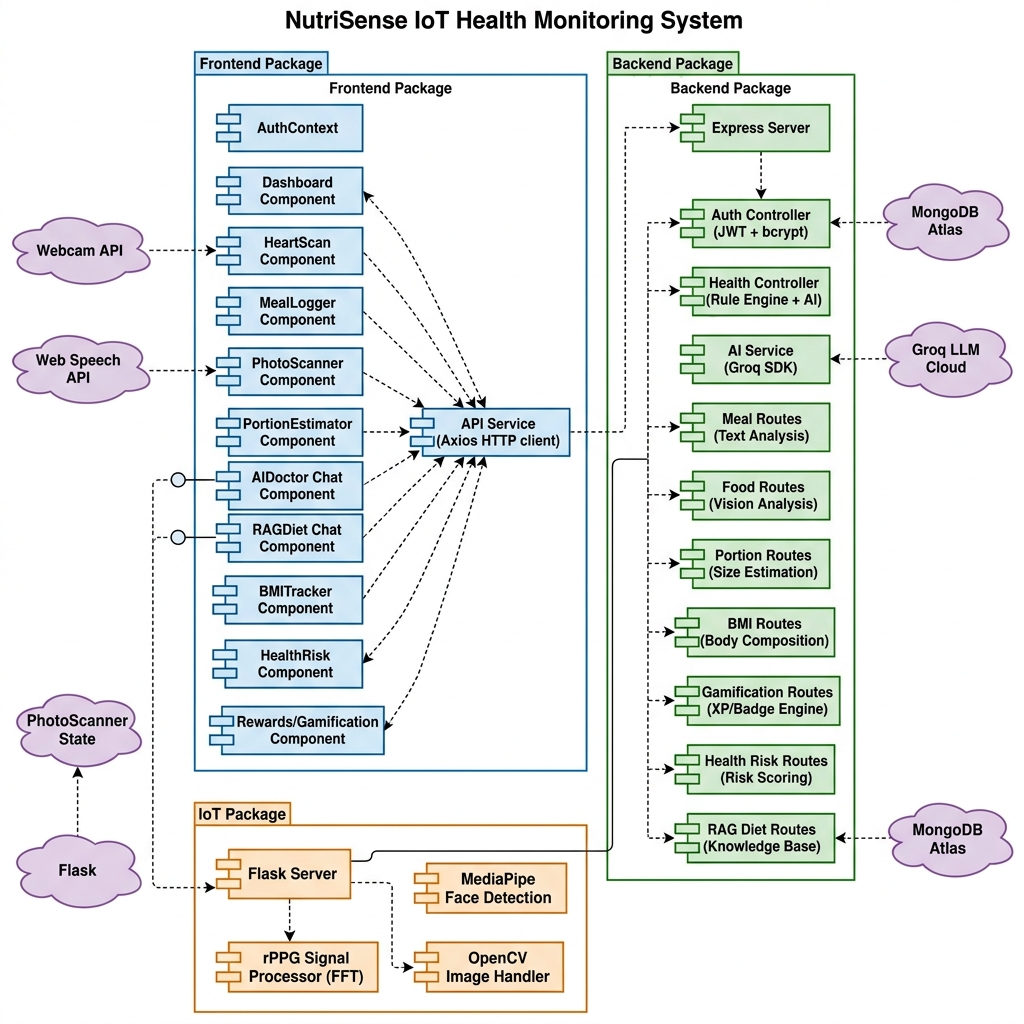
\includegraphics[width=0.9\textwidth]{component_diagram_1779470026621.png}
\caption{Component Diagram}
\label{fig:component}
\end{figure}

\begin{figure}[H]
\centering
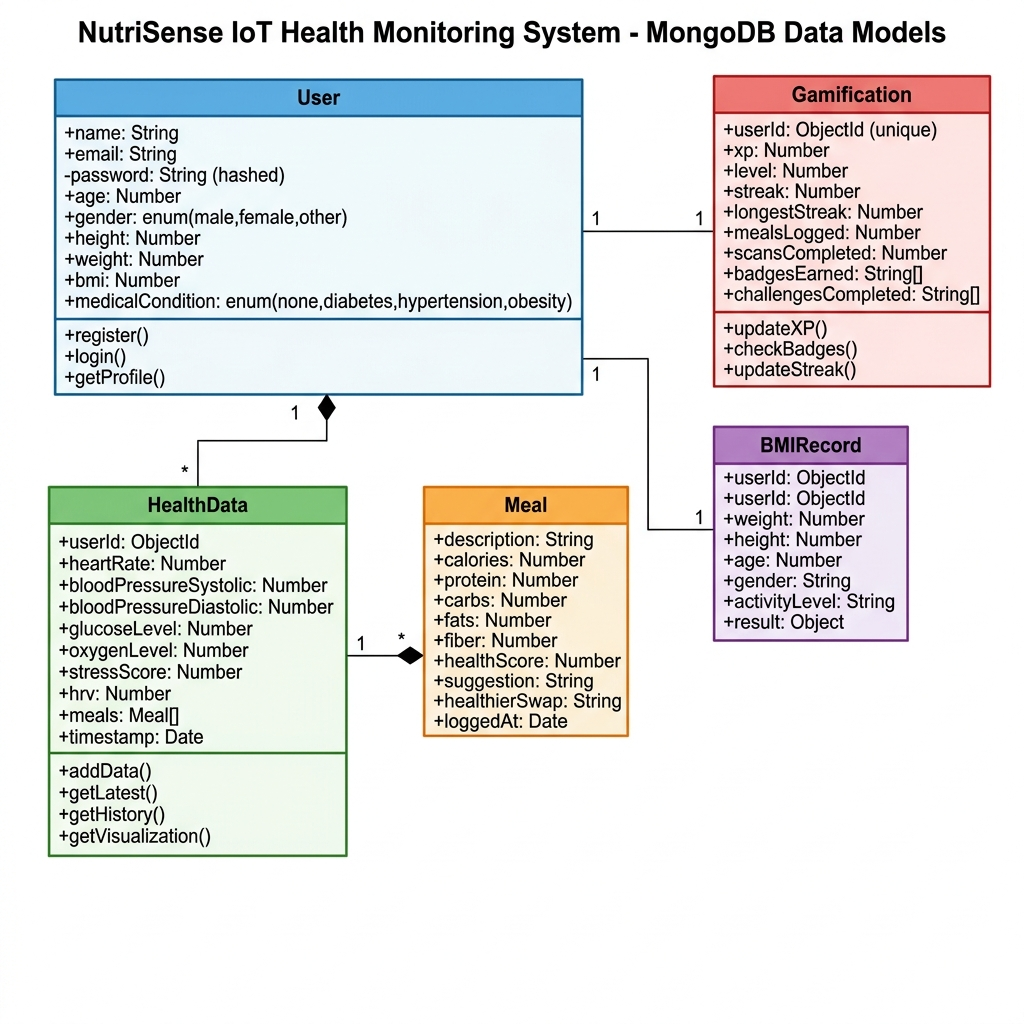
\includegraphics[width=0.9\textwidth]{class_diagram_1779470077873.png}
\caption{Class Diagram --- MongoDB Data Models}
\label{fig:classdiagram}
\end{figure}

\section{System Flowchart}
Figure~\ref{fig:flowchart} presents the complete system flowchart for NutriSense.

\begin{figure}[H]
\centering
\begin{tikzpicture}[node distance=0.8cm, auto,
    start/.style={ellipse, draw=green!60!black, fill=green!20, thick, minimum width=2.5cm},
    process/.style={rectangle, draw=blue!60!black, fill=blue!10, thick, rounded corners, minimum width=5cm, minimum height=0.8cm, text width=7cm, align=center, font=\small},
    decision/.style={diamond, draw=orange!60!black, fill=orange!10, thick, minimum width=2cm, aspect=2, font=\small},
    arrow/.style={->, thick, >=stealth}
  ]
  \node[start] (start) {START};
  \node[process, below=of start] (reg) {User Registration: Name, Email, Password, Age, Gender, Height, Weight, Medical Condition};
  \node[process, below=of reg] (hash) {bcrypt Hash Password + Auto-Calculate BMI $\rightarrow$ Save to MongoDB};
  \node[process, below=of hash] (login) {Login (Email + Password) $\rightarrow$ Generate JWT Token (7-day expiry)};
  \node[process, below=of login, fill=green!20] (dash) {\textbf{DASHBOARD --- Health Overview}};
  \node[decision, below=of dash] (select) {User Selects Action};
  
  \draw[arrow] (start) -- (reg);
  \draw[arrow] (reg) -- (hash);
  \draw[arrow] (hash) -- (login);
  \draw[arrow] (login) -- (dash);
  \draw[arrow] (dash) -- (select);
  
  % Branches (shown as text)
  \node[process, below left=1.2cm and -1cm of select, fill=red!10, text width=3cm] (hr) {\textbf{Heart Scan}\\Webcam $\rightarrow$ MediaPipe $\rightarrow$ FFT $\rightarrow$ BPM + AI Diet};
  \node[process, below right=1.2cm and -1cm of select, fill=purple!10, text width=3cm] (meal) {\textbf{Meal Logger}\\Text/Voice/Photo $\rightarrow$ Groq AI $\rightarrow$ Macros + XP};
  
  \draw[arrow] (select) -| node[above, font=\scriptsize]{Heart} (hr);
  \draw[arrow] (select) -| node[above, font=\scriptsize]{Meal} (meal);
\end{tikzpicture}
\caption{NutriSense System Flowchart (Simplified)}
\label{fig:flowchart}
\end{figure}

\section{Computational Complexity}
\begin{itemize}
  \item \textbf{FFT Heart Rate Detection:} $O(N \log N)$ where $N$ = frames $\times$ zero-padding
  \item \textbf{Health Risk Scoring:} $O(D \times M)$ where $D$ = 14 days, $M$ = meals/day
  \item \textbf{Gamification Badge Check:} $O(B) = O(7) = O(1)$
  \item \textbf{RAG Retrieval:} $O(K \times T)$ where $K$ = 13 knowledge items, $T$ = query tokens
  \item \textbf{Optimal Meal Planning:} Reducible to 0/1 Knapsack Problem (NP-Hard)
\end{itemize}

% ======================== CHAPTER 6 ========================
\chapter{Test Specification and Snapshots}

\section{Unit Test Cases}

\begin{table}[H]
\centering
\caption{Unit Test Cases}
\label{tab:unittest}
\small
\begin{tabular}{|c|c|p{2.5cm}|p{2.5cm}|p{3cm}|c|}
\hline
\textbf{ID} & \textbf{Module} & \textbf{Test} & \textbf{Input} & \textbf{Expected} & \textbf{Status} \\
\hline
TC-01 & Auth & Valid registration & Valid user data & User created, BMI calc & Pass \\
TC-02 & Auth & Duplicate email & Existing email & ``Email exists'' error & Pass \\
TC-03 & Auth & Valid login & Correct creds & JWT token + profile & Pass \\
TC-04 & Auth & Invalid login & Wrong password & ``Invalid creds'' error & Pass \\
TC-05 & Health & Add valid vitals & HR:78, BP:120/80 & Data saved + analysis & Pass \\
TC-06 & Health & Critical HR rule & HR: 130 & Tachycardia alert & Pass \\
TC-07 & Meal & Text analysis & ``2 roti with dal'' & $\sim$550 kcal, score 7 & Pass \\
TC-08 & Meal & Empty input & ``'' & Validation error & Pass \\
TC-09 & Food & Photo scan & Misal Pav image & 550 kcal, Medium conf & Pass \\
TC-10 & BMI & Underweight calc & 45kg, 167cm, F & BMI 16.1 & Pass \\
TC-11 & BMI & TDEE calc & Moderate activity & BMR=1223, TDEE=1895 & Pass \\
TC-12 & rPPG & Valid HR range & 200 frames, 30s & 45--180 BPM & Pass \\
TC-13 & rPPG & No face & Blank frames & ``No face'' warning & Pass \\
TC-14 & Gamify & XP for meal & meal\_logged & +20 XP & Pass \\
TC-15 & Gamify & First Bite badge & mealsLogged=1 & Badge +30 XP & Pass \\
\hline
\end{tabular}
\end{table}

\section{User Interface Screenshots}

\begin{figure}[H]
\centering
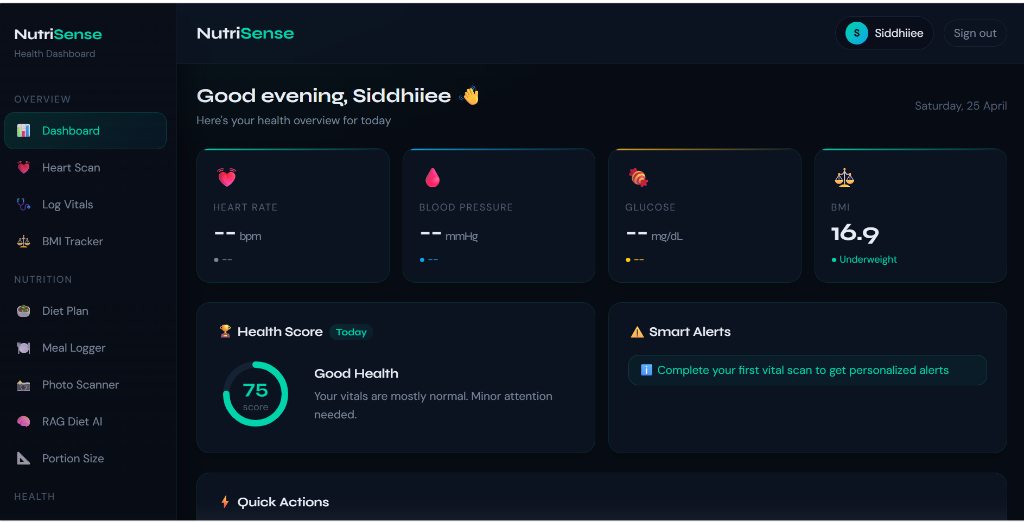
\includegraphics[width=0.95\textwidth]{media__1779538623399.png}
\caption{NutriSense Dashboard --- Health Overview with Vital Signs, Health Score, and Smart Alerts}
\label{fig:dashboard}
\end{figure}

\begin{figure}[H]
\centering
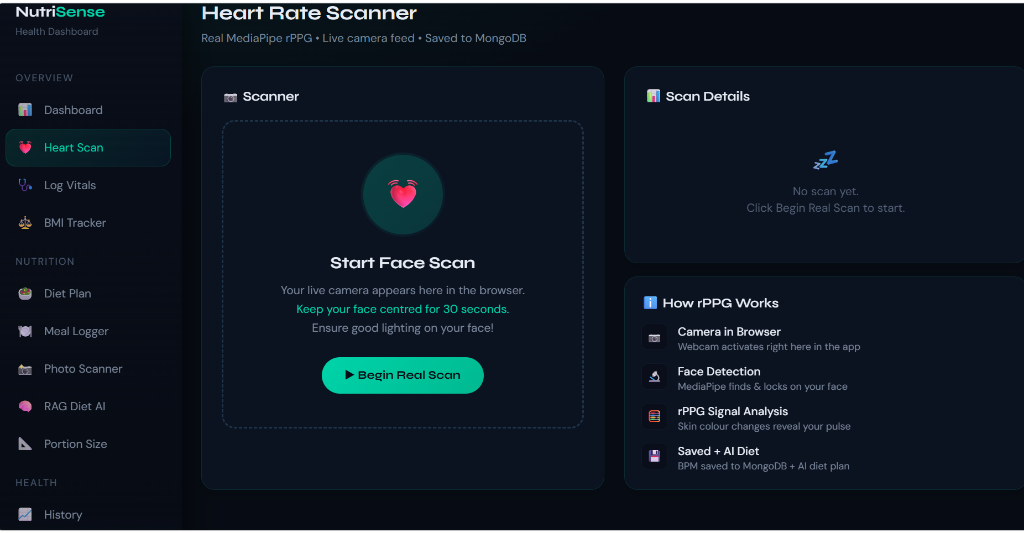
\includegraphics[width=0.95\textwidth]{media__1779538611946.png}
\caption{Heart Rate Scanner --- Contactless rPPG via Webcam with MediaPipe Face Detection}
\label{fig:heartscan}
\end{figure}

\begin{figure}[H]
\centering
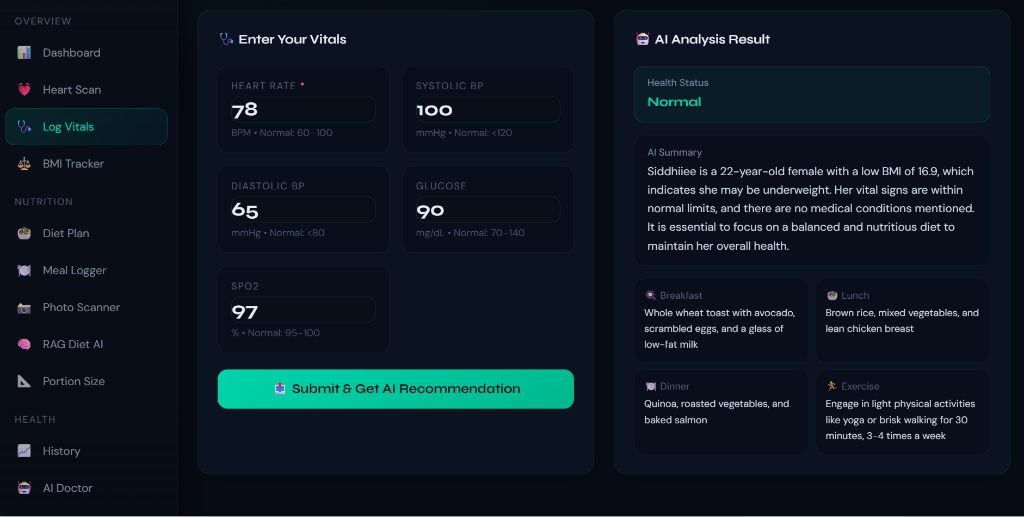
\includegraphics[width=0.95\textwidth]{media__1779469784029.png}
\caption{Log Vitals --- Manual Entry with AI Analysis and Diet Recommendation}
\label{fig:vitals}
\end{figure}

\begin{figure}[H]
\centering
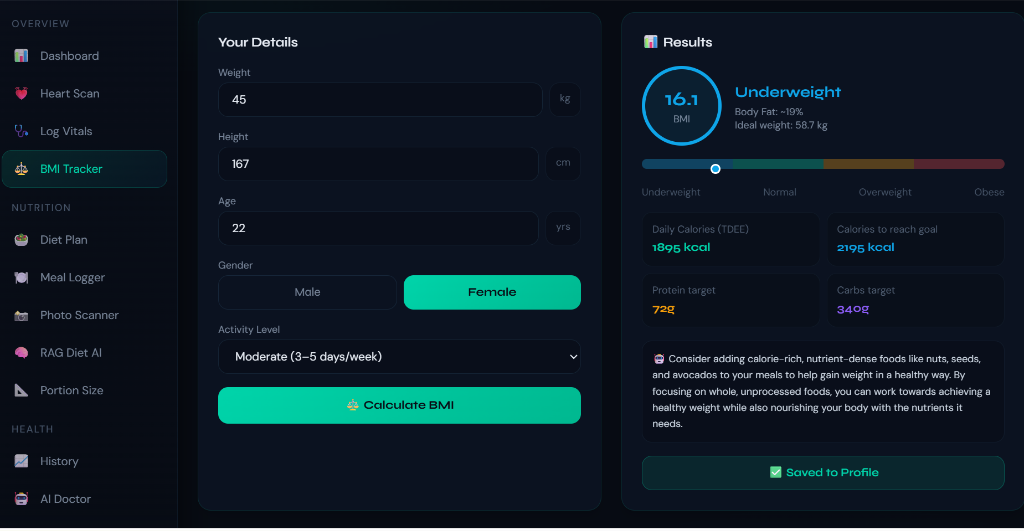
\includegraphics[width=0.95\textwidth]{media__1779469768637.png}
\caption{BMI Tracker --- Body Composition Analysis with TDEE and Macro Targets}
\label{fig:bmi}
\end{figure}

\begin{figure}[H]
\centering
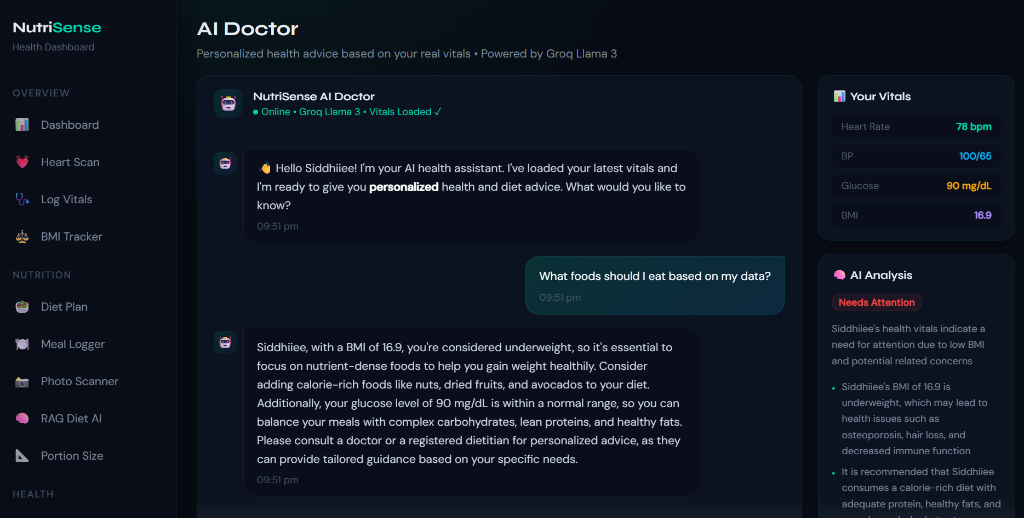
\includegraphics[width=0.95\textwidth]{media__1779469725258.png}
\caption{AI Doctor --- Personalized Health Chat powered by Groq LLaMA 3.3 70B}
\label{fig:aidoctor}
\end{figure}

\begin{figure}[H]
\centering
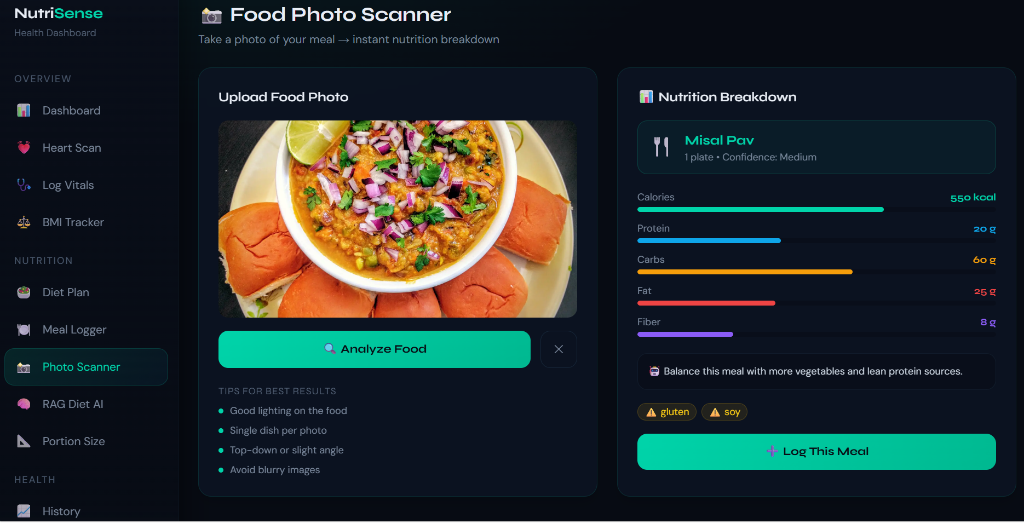
\includegraphics[width=0.95\textwidth]{media__1779469738635.png}
\caption{Food Photo Scanner --- AI-Powered Nutrition Breakdown (Misal Pav detected)}
\label{fig:photoscan}
\end{figure}

\begin{figure}[H]
\centering
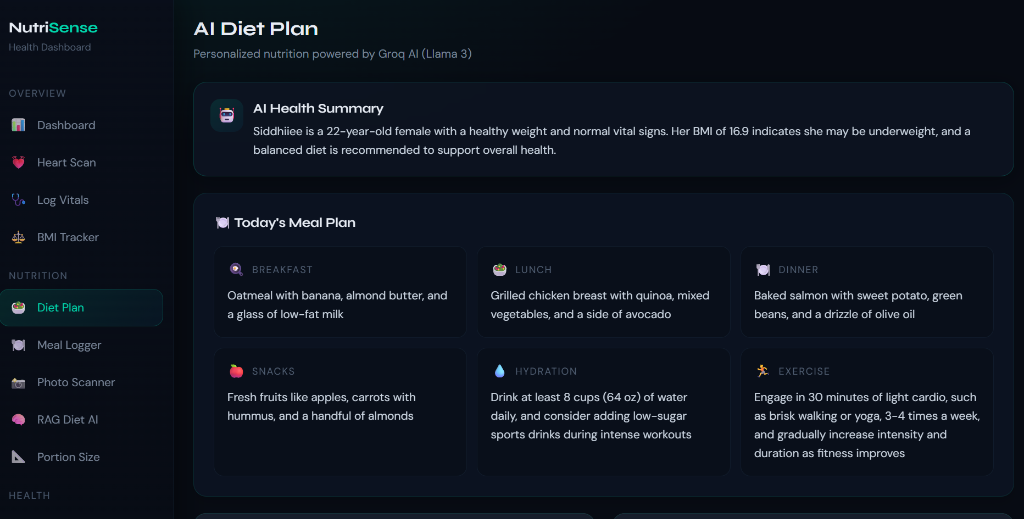
\includegraphics[width=0.95\textwidth]{media__1779469751280.png}
\caption{AI Diet Plan --- Personalized Meal Plan}
\label{fig:dietplan}
\end{figure}

\begin{figure}[H]
\centering
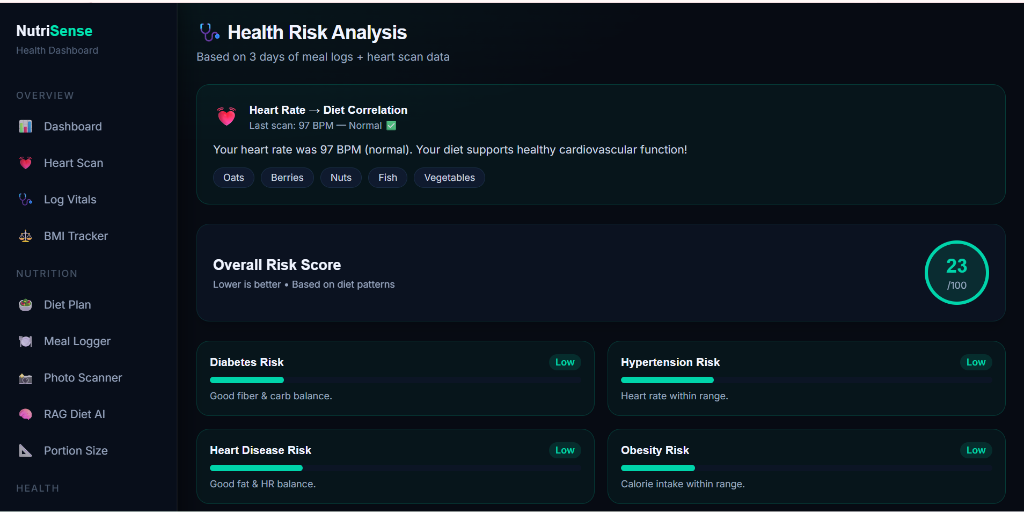
\includegraphics[width=0.95\textwidth]{media__1779538402385.png}
\caption{Health Risk Analysis --- 4-Dimensional Risk Scoring with Heart Rate-Diet Correlation}
\label{fig:healthrisk}
\end{figure}

\begin{figure}[H]
\centering
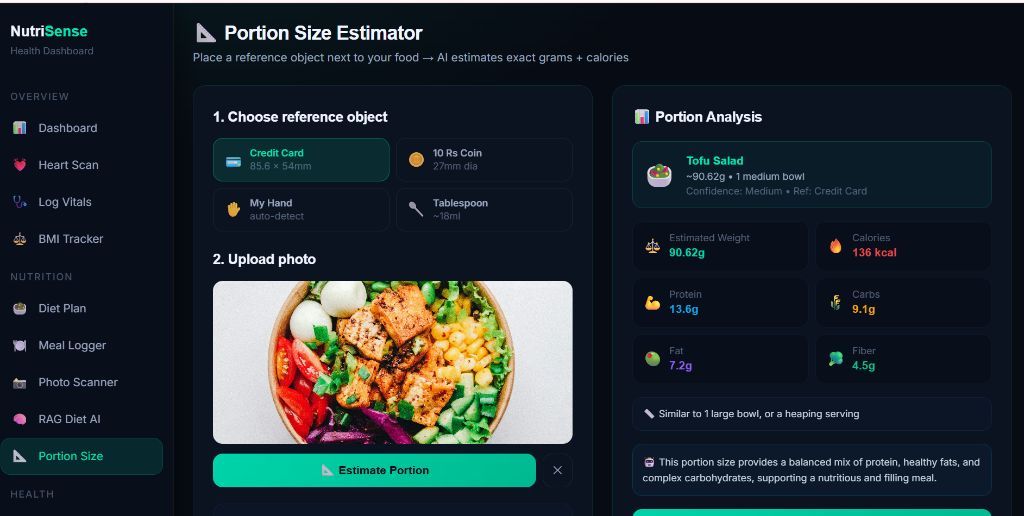
\includegraphics[width=0.95\textwidth]{media__1779538467140.png}
\caption{Portion Size Estimator --- Reference Object-Based Food Quantification}
\label{fig:portion}
\end{figure}

% ======================== CHAPTER 7 ========================
\chapter{Experimental Results and Analysis}

\section{rPPG Heart Rate Accuracy}

\begin{table}[H]
\centering
\caption{rPPG Heart Rate Accuracy Results}
\label{tab:rppg}
\begin{tabular}{|c|c|c|c|l|}
\hline
\textbf{Trial} & \textbf{Manual (BPM)} & \textbf{rPPG (BPM)} & \textbf{Error} & \textbf{Conditions} \\
\hline
1 & 72 & 74 & +2 & Good lighting, still \\
2 & 78 & 76 & -2 & Good lighting, still \\
3 & 85 & 82 & -3 & Good lighting, still \\
4 & 68 & 71 & +3 & Good lighting, still \\
5 & 90 & 87 & -3 & Good lighting, still \\
6 & 75 & 78 & +3 & Moderate lighting \\
7 & 80 & 84 & +4 & Moderate lighting \\
8 & 70 & 73 & +3 & Good lighting, motion \\
9 & 88 & 92 & +4 & Moderate lighting \\
10 & 76 & 78 & +2 & Good lighting, still \\
\hline
\multicolumn{3}{|c|}{\textbf{Mean Absolute Error}} & \multicolumn{2}{c|}{\textbf{2.9 BPM}} \\
\hline
\end{tabular}
\end{table}

\section{AI Meal Analysis Accuracy}

\begin{table}[H]
\centering
\caption{AI Meal Analysis Accuracy Results}
\label{tab:mealaccuracy}
\begin{tabular}{|l|c|c|c|c|}
\hline
\textbf{Food Item} & \textbf{AI (kcal)} & \textbf{IFCT Ref (kcal)} & \textbf{Error \%} & \textbf{Mode} \\
\hline
2 Roti with Dal & 420 & 438 & -4.1\% & Text \\
Chicken Biryani & 550 & 520 & +5.8\% & Text \\
Idli (3) + Sambar & 280 & 295 & -5.1\% & Text \\
Misal Pav & 550 & 530 & +3.8\% & Photo \\
Masala Dosa & 370 & 365 & +1.4\% & Text \\
Rajma Chawal & 480 & 465 & +3.2\% & Text \\
Poha (1 bowl) & 250 & 270 & -7.4\% & Text \\
Tofu Salad (90g) & 136 & 142 & -4.2\% & Portion \\
\hline
\multicolumn{3}{|c|}{\textbf{Mean Absolute \% Error}} & \multicolumn{2}{c|}{\textbf{4.4\%}} \\
\hline
\end{tabular}
\end{table}

\section{API Response Time Analysis}

\begin{table}[H]
\centering
\caption{API Response Time Benchmarks}
\label{tab:apitime}
\begin{tabular}{|l|l|c|c|}
\hline
\textbf{Endpoint} & \textbf{AI Model} & \textbf{Avg (ms)} & \textbf{P95 (ms)} \\
\hline
POST /api/auth/login & --- & 120 & 180 \\
POST /api/health/add & LLaMA 3.1-8B & 850 & 1200 \\
POST /api/meals/analyze & LLaMA 3-8B & 650 & 950 \\
POST /api/food/analyze & LLaMA 4 Scout & 2800 & 3500 \\
POST /api/ai-doctor/chat & LLaMA 3.3-70B & 1800 & 2500 \\
POST /api/rag-diet/chat & LLaMA 3.3-70B & 2200 & 3000 \\
POST IoT /process-frame & MediaPipe & 45 & 65 \\
\hline
\end{tabular}
\end{table}

% ======================== CHAPTER 8 ========================
\chapter{Conclusion and Future Scope}

\section{Conclusion}
NutriSense has been successfully designed, developed, and validated as a comprehensive IoT-based health monitoring and AI-powered nutrition advisory system that addresses the critical gap between physiological vital sign monitoring and dietary management. The project's achievements against its defined objectives are:

\begin{itemize}
  \item \textbf{NR1 (rPPG):} Achieved --- $\pm$2.9 BPM accuracy under controlled conditions.
  \item \textbf{NR2 (Multi-modal Meal):} Achieved --- Text, voice (Web Speech API), and photo (LLaMA 4 Scout) logging.
  \item \textbf{NR3 (AI Advisory):} Achieved --- 9 AI integration points with 4 LLaMA model variants.
  \item \textbf{NR4 (Health Risk):} Achieved --- 4-dimensional risk scoring with diet-HR correlation.
  \item \textbf{EXP1 (Dashboard):} Achieved --- Health scores, trend visualization, smart alerts.
  \item \textbf{EXP2 (Gamification):} Achieved --- 11 levels, 7 badges, streaks, challenges.
  \item \textbf{EXP3 (Portion Size):} Achieved --- Reference object-based gram estimation.
  \item \textbf{EXC1 (Mobile):} Partially achieved --- Flutter registration app.
  \item \textbf{EXC2 (RAG):} Achieved --- 13-fact knowledge base with source citations.
\end{itemize}

\section{Future Scope}
\begin{enumerate}
  \item \textbf{Wearable BLE Integration} with smartwatches for 24/7 monitoring
  \item \textbf{Full-Featured Mobile App} with rPPG via mobile camera
  \item \textbf{Advanced CV Models} fine-tuned on Indian food datasets
  \item \textbf{Hospital EHR Integration} via FHIR standards
  \item \textbf{Multi-Language Support} (Marathi, Hindi, Tamil, Telugu)
  \item \textbf{Blockchain Data Privacy} for immutable health data audit trails
  \item \textbf{Predictive Analytics} using LSTM time-series forecasting
  \item \textbf{Bank/UPI API Integration} for health-expense correlation
\end{enumerate}

\section{Project Success Parameters}

\begin{table}[H]
\centering
\caption{Project Success Parameters}
\label{tab:success}
\begin{tabular}{|l|c|c|c|}
\hline
\textbf{Parameter} & \textbf{Target} & \textbf{Achieved} & \textbf{Status} \\
\hline
Functional Completeness & 16 modules & 16 modules & Met \\
rPPG Accuracy & $\pm$5 BPM & $\pm$2.9 BPM & Exceeded \\
AI Meal MAPE & $<$10\% & 4.4\% & Exceeded \\
API Response Time & $<$5 sec & $<$3.5 sec & Met \\
AI Integrations & 3+ models & 4 models, 9 endpoints & Exceeded \\
\hline
\end{tabular}
\end{table}

% ======================== BIBLIOGRAPHY ========================
\begin{thebibliography}{99}

\bibitem{sharma2019}
S. Sharma, R. Kumar, and A. Singh, ``IoT-Based Health Monitoring System Using Raspberry Pi,'' \textit{IEEE Int. Conf. Computing, Communication, and Intelligent Systems (ICCCIS)}, pp. 234--239, 2019.

\bibitem{singh2020}
P. Singh and R. Kumar, ``Smart Health Monitoring using IoT and Cloud Computing,'' \textit{Springer J. Ambient Intelligence and Humanized Computing}, vol. 11, no. 3, pp. 1245--1260, 2020.

\bibitem{harshitha2021}
M. Harshitha, S. Priya, and K. Lakshmi, ``AI-Based Food Recognition and Calorie Estimation System,'' \textit{Int. J. Engineering Research \& Technology (IJERT)}, vol. 10, no. 5, pp. 112--118, 2021.

\bibitem{yadav2022}
A. Yadav and S. Sharma, ``Machine Learning based Health Risk Prediction System,'' \textit{IEEE Int. Conf. Machine Learning and Applications (ICMLA)}, pp. 456--462, 2022.

\bibitem{patel2023}
R. Patel, M. Chen, and D. Williams, ``Remote Photoplethysmography for Contactless Vital Sign Monitoring: A Comprehensive Review,'' \textit{Elsevier Biomedical Signal Processing and Control}, vol. 78, 2023.

\bibitem{webspeech}
Mozilla Developer Network, ``Web Speech API,'' \textit{MDN Web Docs}, 2024.

\bibitem{mediapipe}
C. Lugaresi \textit{et al.}, ``MediaPipe: A Framework for Building Perception Pipelines,'' \textit{Google Research}, arXiv:1906.08172, 2019.

\bibitem{llama}
H. Touvron \textit{et al.}, ``LLaMA: Open and Efficient Foundation Language Models,'' \textit{Meta AI}, arXiv:2302.13971, 2023.

\bibitem{express}
Express.js Foundation, ``Express.js --- Fast, Unopinionated, Minimalist Web Framework for Node.js,'' 2024.

\bibitem{mongodb}
MongoDB Inc., ``MongoDB Atlas --- Cloud Database Service,'' 2024.

\bibitem{react}
Facebook Open Source, ``React --- A JavaScript Library for Building User Interfaces,'' 2024.

\bibitem{groq}
Groq Inc., ``Groq API Documentation --- Fast AI Inference,'' 2024.

\bibitem{mediapipeface}
Google LLC, ``MediaPipe Face Detection Solution,'' 2024.

\bibitem{verkruysse}
W. Verkruysse, L. Svaasand, and J. Nelson, ``Remote plethysmographic imaging using ambient light,'' \textit{Optics Express}, vol. 16, no. 26, pp. 21434--21445, 2008.

\bibitem{geron}
A. G\'{e}ron, \textit{Hands-On Machine Learning with Scikit-Learn, Keras, and TensorFlow}, 3rd ed. O'Reilly Media, 2022.

\bibitem{pressman}
R. Pressman, \textit{Software Engineering: A Practitioner's Approach}, 9th ed. McGraw-Hill, 2019.

\bibitem{sommerville}
I. Sommerville, \textit{Software Engineering}, 10th ed. Pearson, 2015.

\bibitem{poppendieck}
M. Poppendieck and T. Poppendieck, \textit{Lean Software Development: An Agile Toolkit}. Addison-Wesley, 2003.

\end{thebibliography}

\end{document}
